\documentclass[12pt,letterpaper]{article}

\usepackage[top=1.5in, bottom=1.25in, left=1.25in, right=1.25in]{geometry}
\usepackage{lscape}
\usepackage{graphicx}
\usepackage{geometry}
\usepackage{url}
\usepackage{amsmath}
\usepackage{multirow}
\usepackage{epstopdf}
\usepackage{float}
\usepackage{hyperref}
%%%\linespread{1.1}


\begin{document}

\title{TopPIC-server User Manual}

\author{}

\date{}

\maketitle


\section{Installation}

No installation is needed for TopPIC-server. 
Just download the zip file and unzip it, then you will find
all files shown below. In most cases, we only use the last three files:
\textbf{startup.bat} and \textbf{shutdown.bat} are used to start up and shut down
the server respectively; the last one is the web link for the service.

\begin{figure}[H]
\begin{center}
    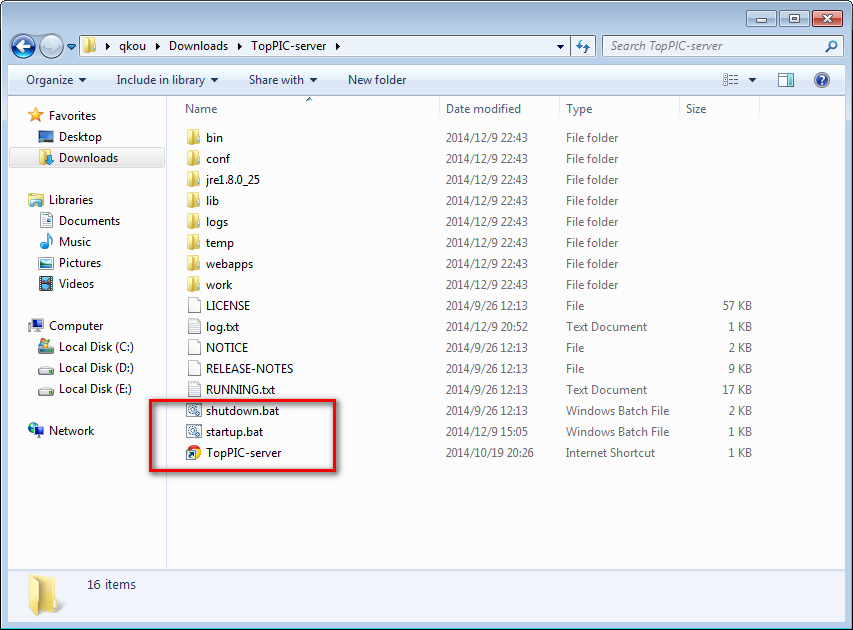
\includegraphics[width=0.9\textwidth]{fig/2.png}
\end{center}
\end{figure}

\section{Start up the server}

To start the TopPIC-server, please double click the ``startup''.
A command line console like below will pop out, 
which means the server begins to run.
You can close the console window and the server will be running in background
until you shut it down.

\begin{figure}[H]
\begin{center}
    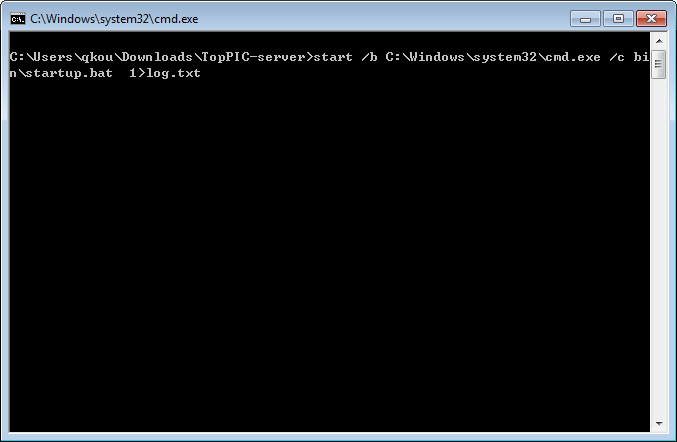
\includegraphics[width=0.6\textwidth]{fig/3.png}
\end{center}
\end{figure}

Also, the web page \url{http://localhost:8080/TopPIC} will be opened.
You can bookmark the web page or use the link we provide in the folder.
It will take more time for the first-time startup due to the service deployment.

\begin{figure}[H]
\begin{center}
    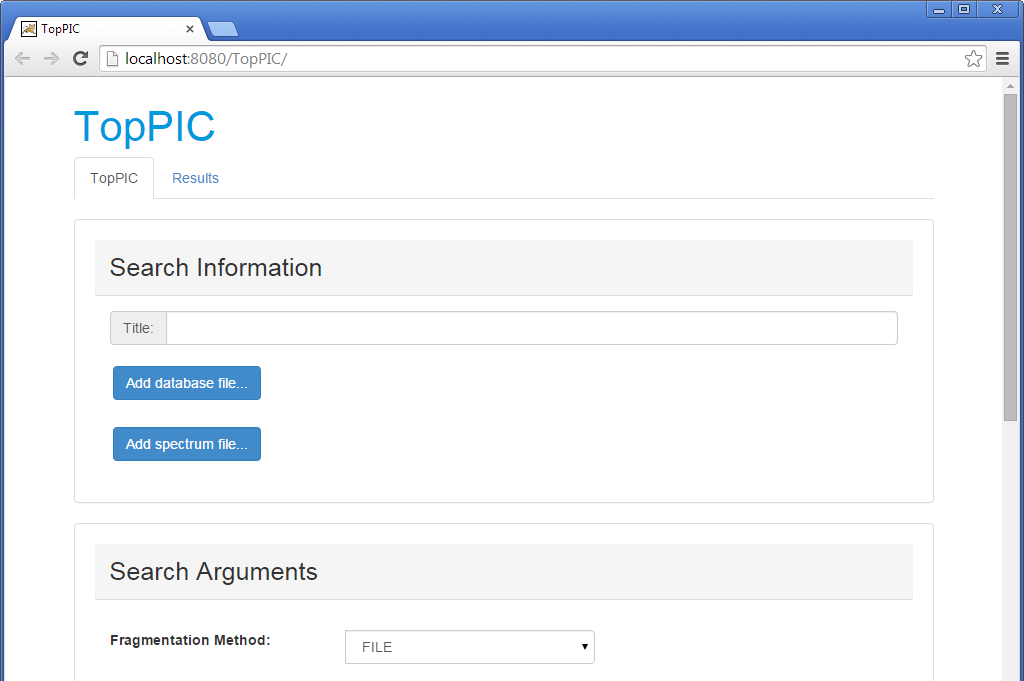
\includegraphics[width=0.8\textwidth]{fig/4.png}
\end{center}
\end{figure}

\section{Submit tasks}

The web page is used to submit tasks and view task status.
In submitting task, you need to provide the task title and upload database
and spectrum file in \textbf{Search Information} part. Only \textbf{fasta} 
format is accepted for database and \textbf{msalign} format for spectrum file.

\begin{figure}[H]
\begin{center}
    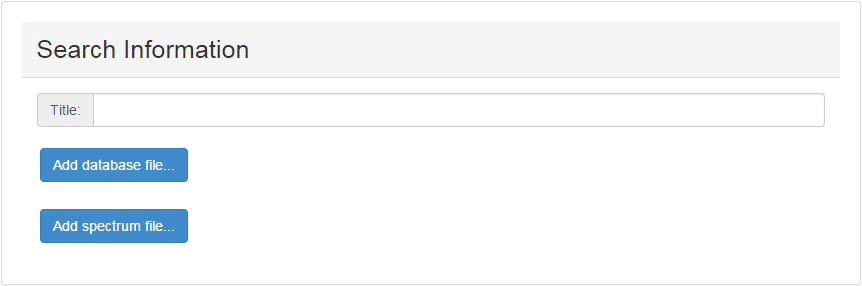
\includegraphics[width=0.9\textwidth]{fig/5.png}
\end{center}
\end{figure}

You can set searching arguments in \textbf{Search Arguments} part. Detailed
explanation is provided below.

\begin{figure}[H]
\begin{center}
    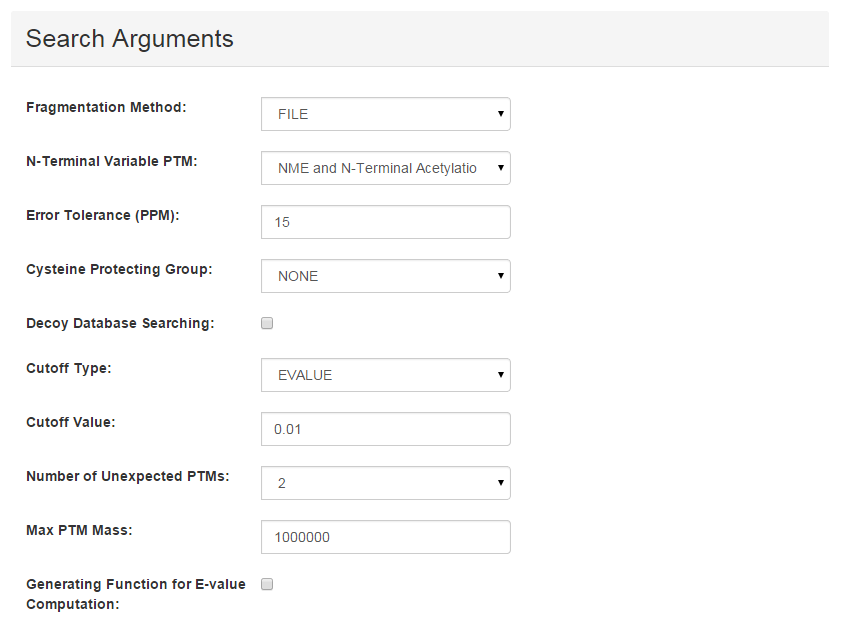
\includegraphics[width=0.9\textwidth]{fig/6.png}
\end{center}
\end{figure}

\begin{itemize}
\item Fragmentation Method. Four options are provided: FILE, CID, ETD, HCD. The
default value is FILE, which means getting fragmentation method from the
spectrum file.
\item N-Terminal Variable PTM. Three options are provided: NME and N-Terminal Acetylation, NONE, NME.
\item Error Tolerance (PPM). Error tolerance for precursor and fragment masses 
in parts per million.
\item Cysteine Protecting Group. Three options are provided: NONE, 
Carbamidomethylation (C57), Carboxymethylation (C58). The default value is NONE.
\item Decoy Database Searching. When selected, a shuffled decoy protein database
will be used to estimate false discovery rates.
\item Cutoff Type. The cutoff type are support: EVALUE and FDR. The Decoy Database Searching option must be selected, if you want to use FDR.
\item Cutoff Value. Cutoff value for reporting proteoform-spectrum-matches.
\item Number of Unexpected PTMs. Maximum number of unexpected post-translational modifications in a proteoform-spectrum-match.
\item Max PTM Mass. Maximum absolute value of masses (in Dalton) of unexpected post-translational modifications in proteoforms.
\item Fast E-values Estimation. When selected, precomputed estimation will be
used to save time. The error tolerance can only be 15, 10, or 5 when this option
selected.
\end{itemize}

After setting basic information and searching arguments, you can submit
the task. If all the information and arguments are valid, you can submit 
another task or check the task status.

\begin{figure}[H]
\begin{center}
    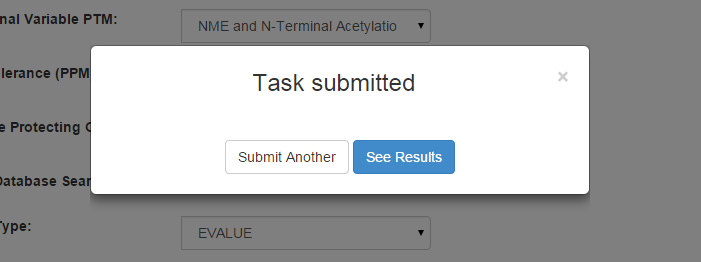
\includegraphics[width=0.8\textwidth]{fig/7.png}
\end{center}
\end{figure}

\section{View task status}

In the results tab, you can view the information about all the tasks submitted,
including id, title, submission time, running time and progress.
You can refresh the running progress, stop running task and delete waiting task
by using corresponding buttons.

\begin{figure}[H]
\begin{center}
    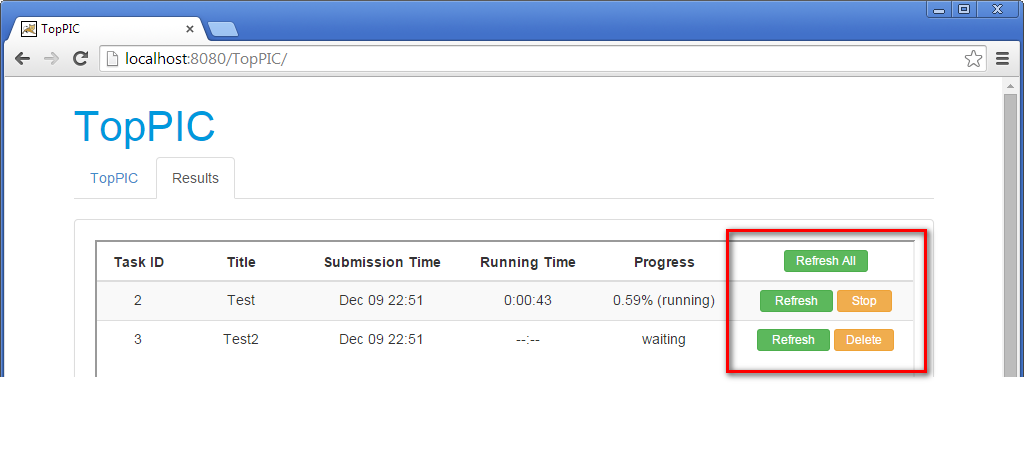
\includegraphics[width=0.9\textwidth]{fig/8.png}
\end{center}
\end{figure}

\section{Download searching results}

You can find the download button for each finished and stopped task.


\begin{figure}[H]
\begin{center}
    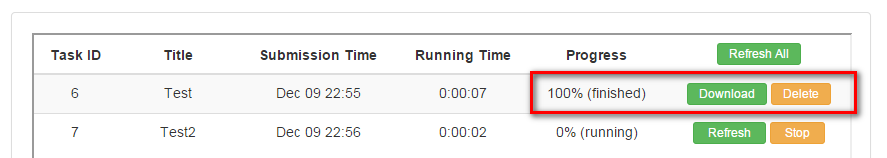
\includegraphics[width=0.9\textwidth]{fig/9.png}
\end{center}
\end{figure}

The task result will be packaged into a zip file and you can download it
using the link we provide.
It may take some time for zipping all the results.

\begin{figure}[H]
\begin{center}
    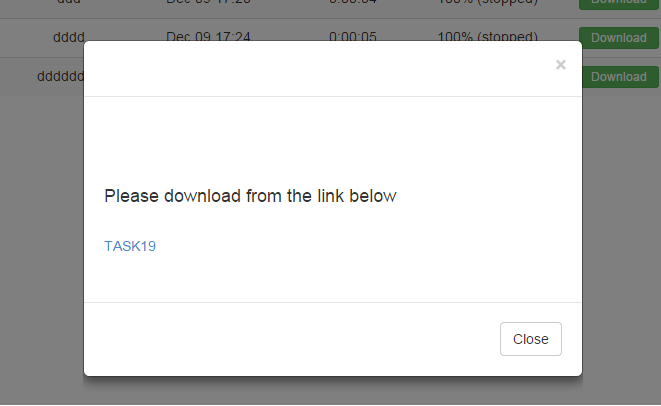
\includegraphics[width=0.8\textwidth]{fig/10.png}
\end{center}
\end{figure}

The result contains a tab delimited text file and a collection of html files for identified proteoforms.
For example, when the input spectral data file is spectral.msalign, 
the tab delimited text file is spectral.OUTPUT\_TABLE and 
the html files are in the directory spectral\_html. 
Use a web browser, such as Chrome or Firefox, 
to open the file spectral\_html/proteins.html to browse all identified proteoforms.

The result of 
\href{http://proteomics.informatics.iupui.edu/software/toppic/ST/proteins.html}{\textit{Salmonella typhimurium}} and
\href{http://proteomics.informatics.iupui.edu/software/toppic/EC/proteins.html}{\textit{Escherichia coli}}
data sets are shown as examples.



\end{document}
